\documentclass{beamer}
\usepackage[french]{babel}
\usepackage[utf8]{inputenc}
\usepackage[T1]{fontenc}
\usepackage{multirow}
\usepackage{graphicx}
\usepackage{tikz}
\usepackage{hyperref}
\usepackage[linguistics]{forest}

\title{CrashCoin}
\subtitle{Une crypto-monnaie qui ne vaut rien}
\author{Rémy~Detobel \and Stanislas~Gueniffey \and Denis~Hoornaert \and Nathan~Liccardo \and Antoine~Passemiers \and Robin~Petit \and Alexis~Reynouard \and Cedric~Simar}
\institute{Université Libre de Bruxelles}
\subject{Sujet}
\usetheme{Singapore} %It's beautiful and neat, why change it ?
\usecolortheme{whale}
\usepackage[footheight=1em]{beamerthemeboxes}

\usebackgroundtemplate{\tikz\node[opacity=0.15] {
\includegraphics[height=\textheight]{logo.png}};}
 
%bibliography
\setbeamertemplate{bibliography item}{}
\setbeamertemplate{bibliography entry title}{}
\setbeamertemplate{bibliography entry location}{}
\setbeamertemplate{bibliography entry note}{}
 
\addfootboxtemplate{}{\color{white}
\hfill\insertframenumber\hspace{1em}}
\setbeamertemplate{navigation symbols}{}


\begin{document}
\maketitle
\nocite{*} %Display all references without need to cite

\begin{frame}{Table des matières}
    \tableofcontents
\end{frame}

\section{Introduction}
\begin{frame}{Introduction}
    \begin{itemize}
    	\item CrashCoin est écrit en \texttt{Java 8}
        \item Utilise des librairies cryptographiques de qualité :
        \begin{itemize}
        	\item \texttt{Java Standard Edition Security 8}
            \item \texttt{Java Cryptography Extension 8}
            \item \texttt{Bouncy Castle 1.57}
        \end{itemize}
    \end{itemize}
\end{frame}

\section{Structure}
\begin{frame}{Structure du projet}
    Nous avons divisé le projet en quatre parties : 
    \begin{enumerate}
    \item Client
    \item Master
    \item Miner
    \item Relay
    \end{enumerate}
    Auxquelles s'ajoute une cinquième partie commune à toutes les parties.
\end{frame}

\subsection{Client}
\begin{frame}{Client}
    Chaque client a la possibilité de posséder un ou plusieurs Wallets sur sa machine. Le client (unique) n'ouvre cependant qu'un seul Wallet à la fois.
    \begin{center}
    \begin{forest}
    [
    	ClientApplication [
        	[Wallet 1]
            [Wallet 2 \ ...]
            [Wallet n]
        ]
    ]
    \end{forest}
    \end{center}
    Tout client souhaitant recevoir ou envoyer une transaction passe par un Relay qui s'occupera de traiter la transaction.
\end{frame}

\subsection{Relay}
\begin{frame}{Relay}
 Chaque instance de Relay constitue un élément centrale du réseau. Ils disposent des connexions suivantes : 
 \begin{itemize}
 \item \texttt{Master Connection} : connexion directe pour la Blockchain.
 \item \texttt{Miner Connection \& Listener} : échange de transactions et de blocs minés.
 \item \texttt{Wallet Connection \& Listener} : envoi et réception de transactions.
 \end{itemize}
\end{frame}

\subsection{Miner}
\begin{frame}{Miner}
 Chaque \texttt{Miner} est connecté directement à un \texttt{Relay} :
 \begin{itemize}
 \item \texttt{RelayConnection} : permet de récupérer à partir du \texttt{Relay} les transactions à Miner;
 \item \texttt{Miner} : est découpé en plusieurs tâches
 	\begin{enumerate}
 		\item Trnasactions à miner (\texttt{RelayConnectio.hasTransaction()}).
 		\item Suppression des blocs minés.
        \item Lance le minage et vérifie s'il dispose d'assez de transactions (\texttt{makeBlockAndMineIt}).
 	\end{enumerate}
 \item Tous les blocs sont de tailles équivalentes.
 \end{itemize}
\end{frame}

\subsection{Master}
\begin{frame}{Master}
\end{frame}

\section{Common}
\begin{frame}{Common}
	\texttt{common.utils.Cryptography} contient les fonctions cryptographiques
    \begin{itemize}
    	\item \texttt{hashBytes} calcule le hash de données avec SHA-256
        \item \texttt{deriveKey} dérive l'adresse d'une clé publique avec RIPEMD160
        \item \texttt{signData} crée une signature pour des données avec DSA
    \end{itemize}
\end{frame}

\section{Communications}
\begin{frame}
	\frametitle{Comminucations}
    \framesubtitle{Émission d'une transaction}
    \begin{columns}
      \begin{column}{.5\textwidth}
      	\begin{center}
      		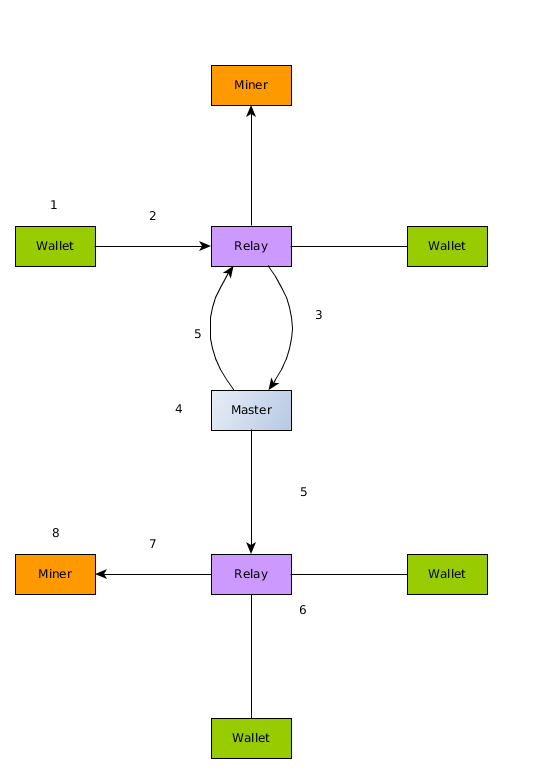
\includegraphics[scale=0.25]{sendTransaction.png}
      	\end{center}
      \end{column}
      \begin{column}{.5\textwidth}
		\begin{enumerate}
			\item \textit{Wallet} signe sa transaction sur base de sa clef privée
            \item La transaction est envoyé a un \textit{relay}
            \item Le \textit{relay} retransmet la transaction à master
            \item \textit{Master} broadcast l'information à tout ses \textit{relay}
            \item 
            \item 
            \item 
            \item 
		\end{enumerate}
      \end{column}
    \end{columns}
\end{frame}

\begin{frame}{Classes communes}
    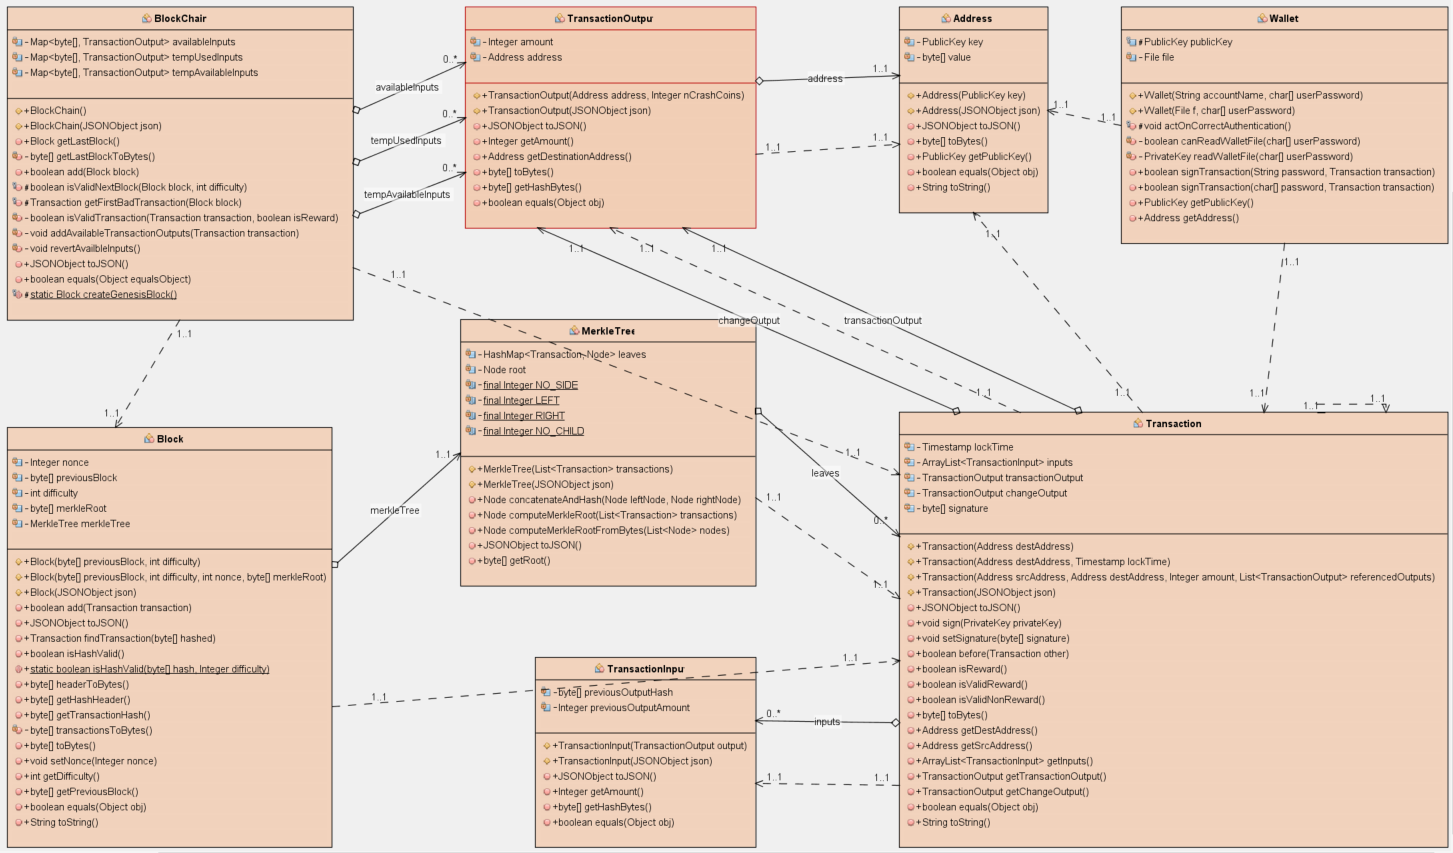
\includegraphics[width=\textwidth]{common-uml.png}
\end{frame}

\begin{frame}{Références}

    {\footnotesize
    	\bibliographystyle{apalike}
		\bibliography{references.bib}
    }
\end{frame}

\end{document}
